\newpage
\subsection{Actividad 12}
Resintonizar el controlador digital respectivamente en
\textsc{SIMULINK} a través de las herramientas de diseño automático,
obteniendo una mejora en la respuesta posible ante seguimiento de
consigna ángulo de amplitud unitaria.

\begin{tcolorbox}[sharp corners, colframe=bluebox, title= Simulink]
  \mkanscode{
\begin{figure}[H]
  \centering
  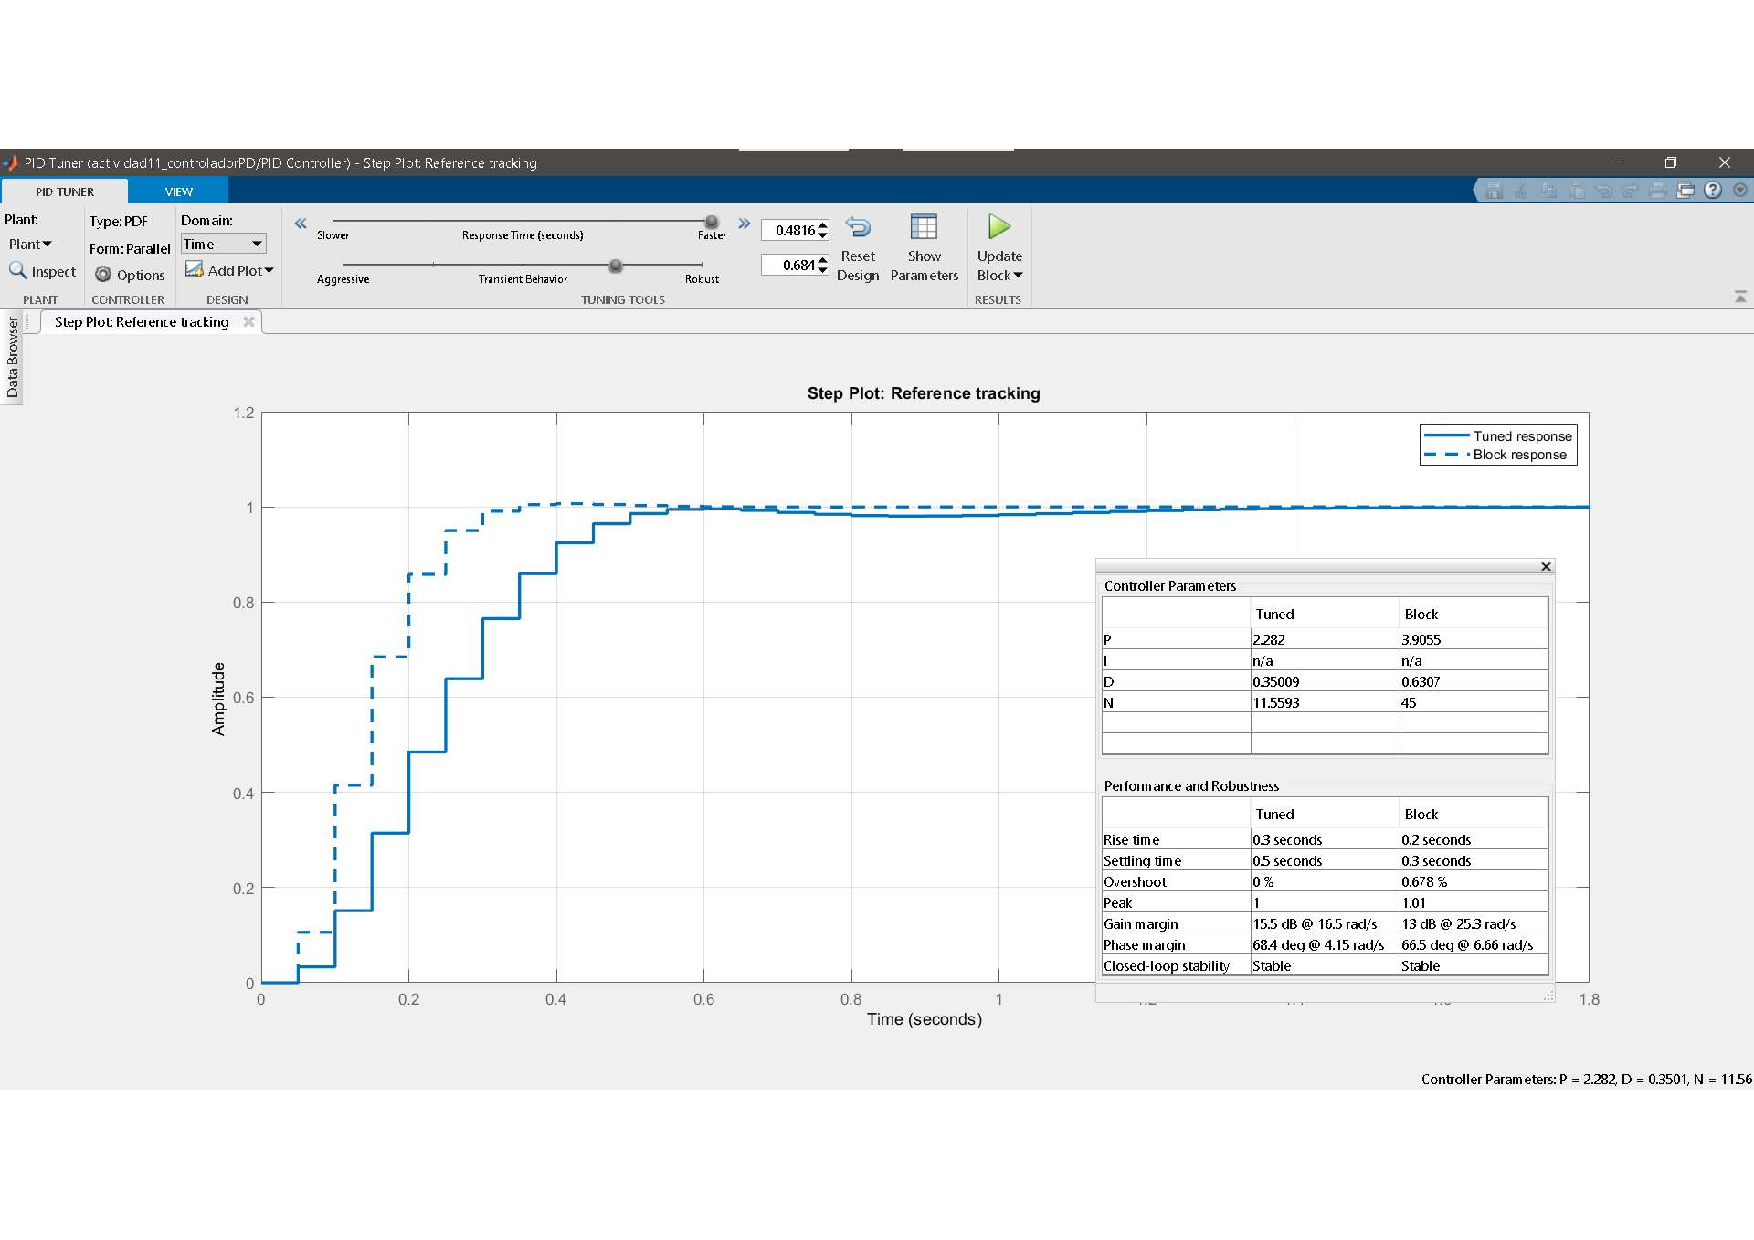
\includegraphics[clip, trim=0cm 2.5cm 0cm 2.5cm,scale=0.45]{images/figura 16.pdf}
  % izquierda,abajo,derecha,arriba
  \caption{Simulink Resintonización PD.}
    \label{fig:figura 16}
\end{figure}
}
\vspace*{0.5em}
  \mkanscode{
\begin{figure}[H]
  \centering
  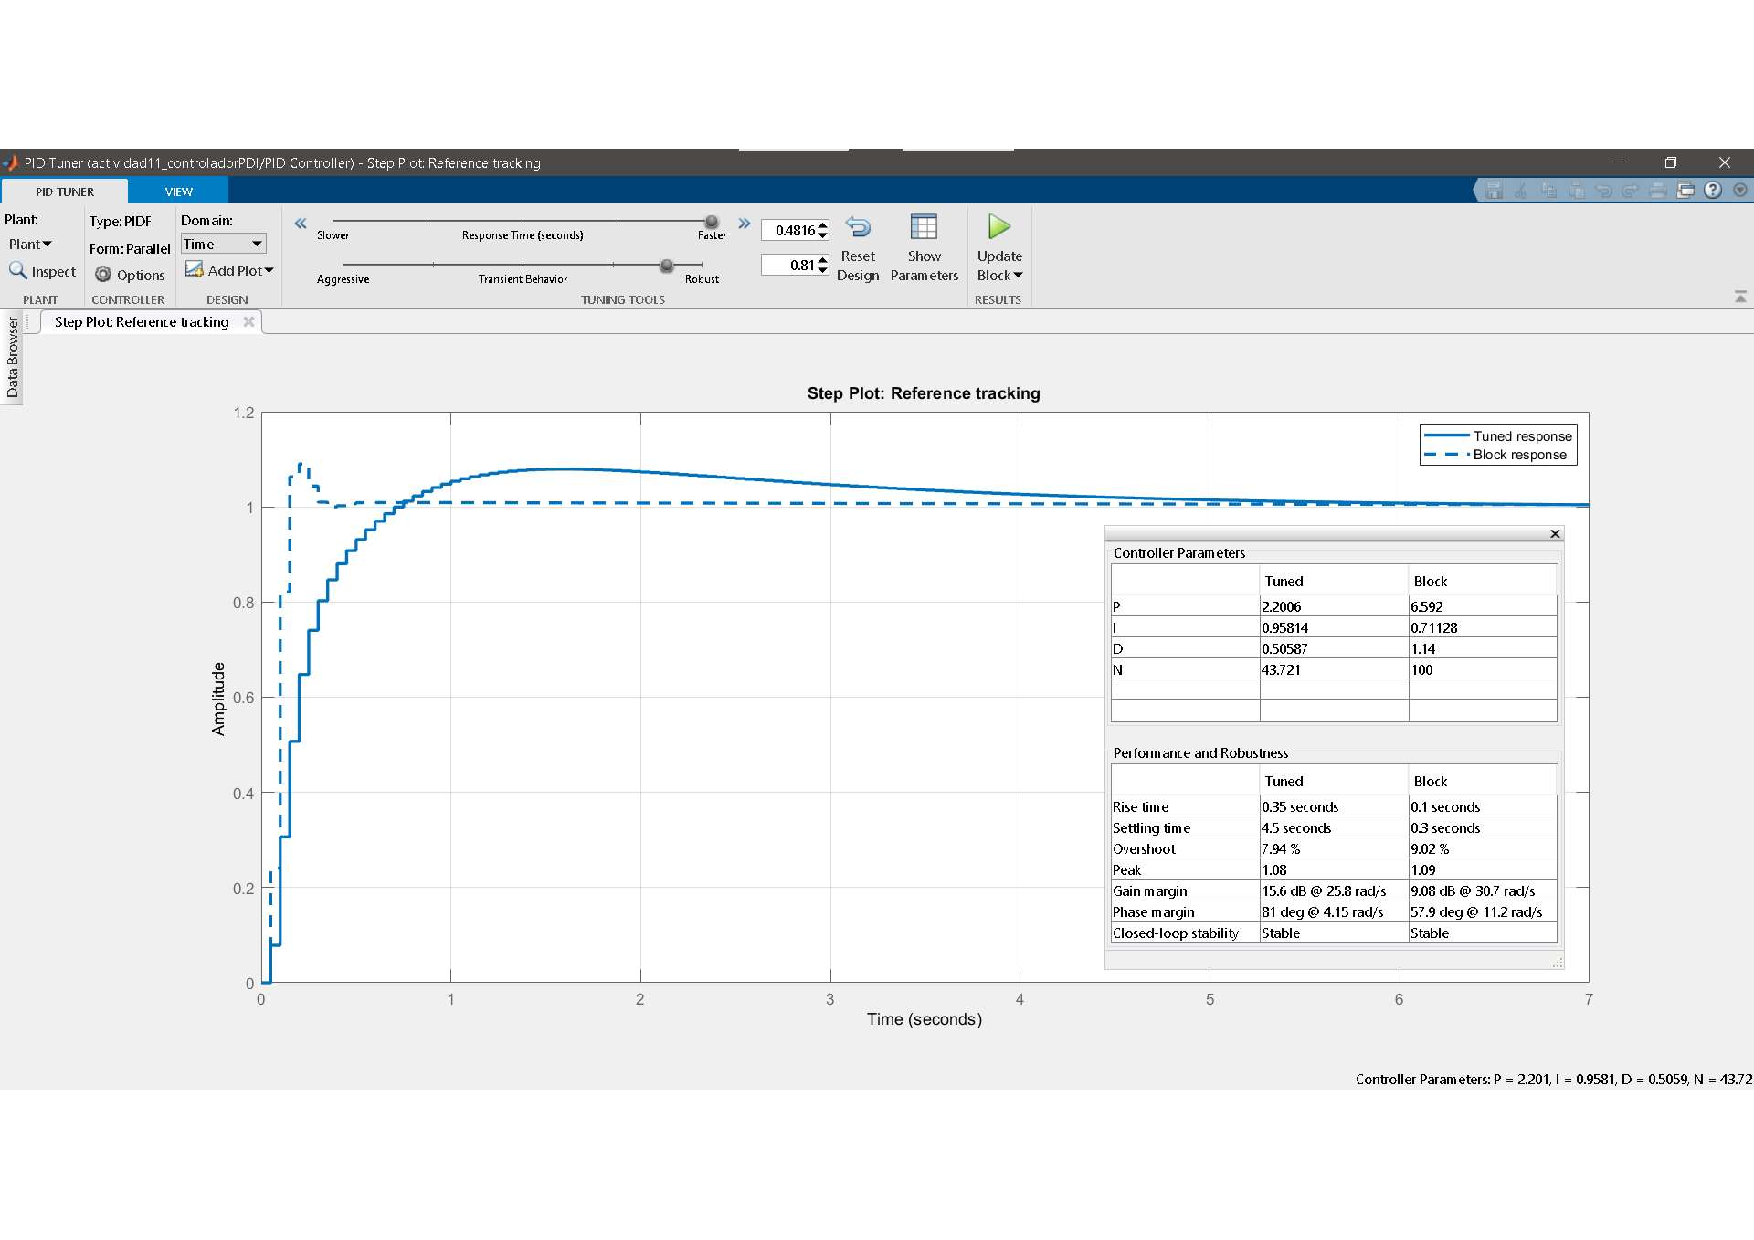
\includegraphics[clip, trim=0cm 2.5cm 0cm 2.5cm,scale=0.45]{images/figura 17.pdf}
  % izquierda,abajo,derecha,arriba
  \caption{Simulink Resintonización PID.}
    \label{fig:figura 17}
\end{figure}
  }
  \end{tcolorbox}%